\documentclass[aspectratio=169]{ctexbeamer}
\definecolor{urls}{RGB}{137, 180, 250}
\definecolor{link_text}{RGB}{245, 224, 220}
\hypersetup{
  colorlinks,
  linkcolor=, % This config controls the jumps inside the pdf
  urlcolor=urls,
}
\renewcommand{\UrlFont}{\ttfamily\scriptsize}

\usetheme{AnnArbor}
\usepackage[style=Mocha,accent=Rosewater]{beamercolorthemecatppuccin}

\usefonttheme{serif}
\usefonttheme{professionalfonts}

\usepackage[T1]{fontenc}
\setmainfont{LXGW WenKai}
% \setmainfont{Cascadia Code NF}
% \setsansfont{}
\setmonofont{Cascadia Code NF}
\usepackage{xeCJK}
\setCJKmainfont{LXGW WenKai}
% \setCJKmainfont{}
\setCJKmonofont{Cascadia Code NF}
\newcommand{\nerd}[1]{\texttt{#1}}
\setmonofont{Cascadia Code NF}[
  Contextuals=Alternate
]

\PassOptionsToPackage{hyphens}{url}
% \usepackage{ulem}
\usepackage{graphicx}
%\usepackage{wrapfig}
\usepackage{pifont} % Symbols used as itemize symbols
\usepackage{enumitem}
\setlist[itemize,1]{label={\small\color[RGB]{242, 205, 205}\ding{111}}}
\setlist[itemize,2]{label={\footnotesize\color[RGB]{242, 205, 205}\ding{111}}}
\usepackage{float}
\usepackage{booktabs}

\setbeamerfont{footnote}{size=\tiny}
\setbeamertemplate{footnote}{%
  \color[RGB]{108, 112, 134}%
  \insertfootnotetext%
}
\setlength{\footnotesep}{0.3\baselineskip}
\newcommand{\refnote}[1]{\footnotetext{#1}}

\usetheme{AnnArbor}

\usepackage{amsmath, amssymb, amsthm}
\usepackage{listings}
\lstdefinestyle{bash}{
  alsoletter=-,
  keywordstyle=[2]{\color[RGB]{243, 139, 168}},
  morekeywords=[2]{sudo},
  keywordstyle=[3]{\color[RGB]{166, 227, 161}},
  morekeywords=[3]{add-apt-repository, apt-get, apt},
  keywordstyle=[4]{\color[RGB]{250, 179, 135}},
  morekeywords=[4]{install},
}
\lstdefinestyle{lua}{
  alsoletter=-,
  keywordstyle=[2]{\color[RGB]{137, 180, 250}},
  morekeywords=[2]{name, priority, opts, config, dependencies, submodules, main, version, init, number, boolean},
  keywordstyle=[3]{\color[RGB]{180, 190, 254}},
  morekeywords=[3]{fun, setup},
  keywordstyle=[4]{\color[RGB]{250, 179, 135}},
  morekeywords=[4]{},
}
\lstdefinestyle{path}{
  alsoletter=~,
  basicstyle={\footnotesize\ttfamily\color[RGB]{147, 153, 178}\itshape},
}
\lstset{
  language={[5.1]lua},
  style=lua,
  basicstyle=\footnotesize\ttfamily,
  breaklines=true,
  showstringspaces=false,
  breakatwhitespace=true,
  keywordstyle=\color[RGB]{245, 169, 127},
  numberstyle={\ttfamily\color[RGB]{110, 115, 141}},
  commentstyle={\color[RGB]{147, 153, 178}\itshape},
  stringstyle={\color[RGB]{166, 218, 149}},
}
% NOTE: \lstinline{} command does not support background color
\lstdefinestyle{nvim}{
  alsoletter=:,
  keywordstyle=[3]{\color[RGB]{166, 227, 161}},
  morekeywords=[3]{:Tutor, :help}, % ChkTeX 26
}

\newcommand{\TODO}[1]{\textcolor{red}{TODO\@: #1} }

% \newcommand{\link}[3][]{\href{#3}{#2}\footnote[#1]{\url{#3}}}
\newcommand{\link}[3][]{\href{#3}{#2\textsuperscript{\nerd{}}}}



\title{Neovim从入门到出门}
\subtitle{第三节:AI补全与对话}
\author{Jacky-Lzx}
\date{\today}

\usepackage{tikz}
\titlegraphic {
  \begin{tikzpicture}[overlay,remember picture]
    \node at (-6, 4.5){
      
\includegraphics[height=1cm]{./Figures/Neovim_logo.png}
    };
    \node at (6, 4.5){
      
\includegraphics[height=1cm]{./Figures/Catppuccin_logo.png}
    };
    \node at (0, 0){
      
\includegraphics[height=0.8cm]{./Figures/Copilot.png}
    };
  \end{tikzpicture}
}

\usepackage{makecell}

\begin{document}

\begin{frame}
  \titlepage
\end{frame}

\begin{frame}{大纲}
  \tableofcontents
\end{frame}
% Current section
\AtBeginSection[ ] {
  \begin{frame}{大纲}
    \tableofcontents[currentsection]
  \end{frame}
}

\section{AI在编程中的使用}
  \begin{frame}{AI在编程中的使用}
    \begin{itemize}
      \item AI补全
        \begin{itemize}
          \item AI根据上下文自动补全代码
          \item 主要插件:\link{copilot.lua}{https://github.com/zbirenbaum/copilot.lua}
        \end{itemize}
      \item AI对话
        \begin{itemize}
          \item 用户跟AI对话,提出要求,AI根据上下文编写代码,完成用户要求
          \item 主要插件:\link{codecompanion.nvim}{https://github.com/olimorris/codecompanion.nvim}
        \end{itemize}
    \end{itemize}
  \end{frame}

\section{插件安装}

  \subsection{copilot.lua}
    \begin{frame}{copilot.lua}
      \begin{itemize}
        \item Copilot订阅
          \begin{itemize}
            \item 如果你是学生,你可以申请\link{Github Student Developer Pack}{https://education.github.com/pack},可以免费使用Copilot % ChkTeX 19
          \end{itemize}
        \item 使用的插件
          \begin{itemize}
            \item \link{copilot.lua}{https://github.com/zbirenbaum/copilot.lua}:利用Copilot提供代码补全
            \item \link{blink-copilot}{https://github.com/fang2hou/blink-copilot}:将Copilot的补全结果显示在blink.cmp中
          \end{itemize}
        \item 安装后的效果
          \begin{figure}[H]
            \centering
            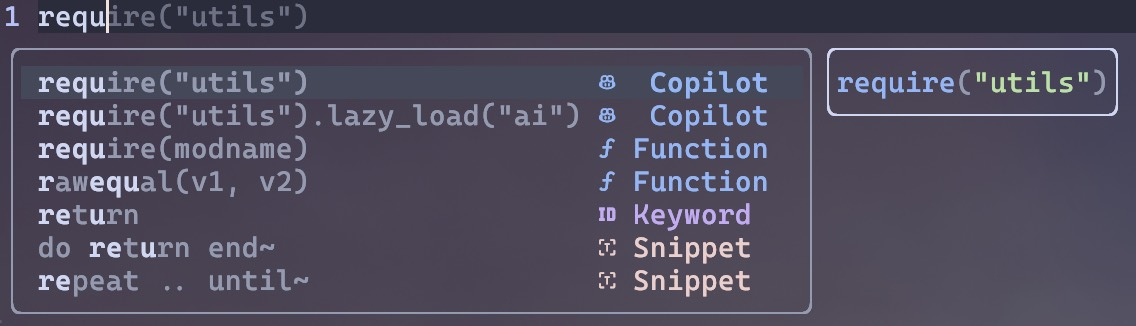
\includegraphics[width=0.6\linewidth]{./Figures/Copilot_Install_Result.jpg}
          \end{figure}
      \end{itemize}
    \end{frame}

  \subsection{codecompanion.nvim}
    \begin{frame}{codecompanion.nvim}
      \begin{itemize}
        \item CodeCompanion使你可以在Neovim中使用大模型帮你修改代码,可以接入多种大模型
        \item 使用的插件
          \begin{itemize}
            \item \link{codecompanion.nvim}{https://github.com/olimorris/codecompanion.nvim}:CodeCompanion本体
          \end{itemize}
        \item 安装后的效果
          \begin{figure}[H]
            \centering
            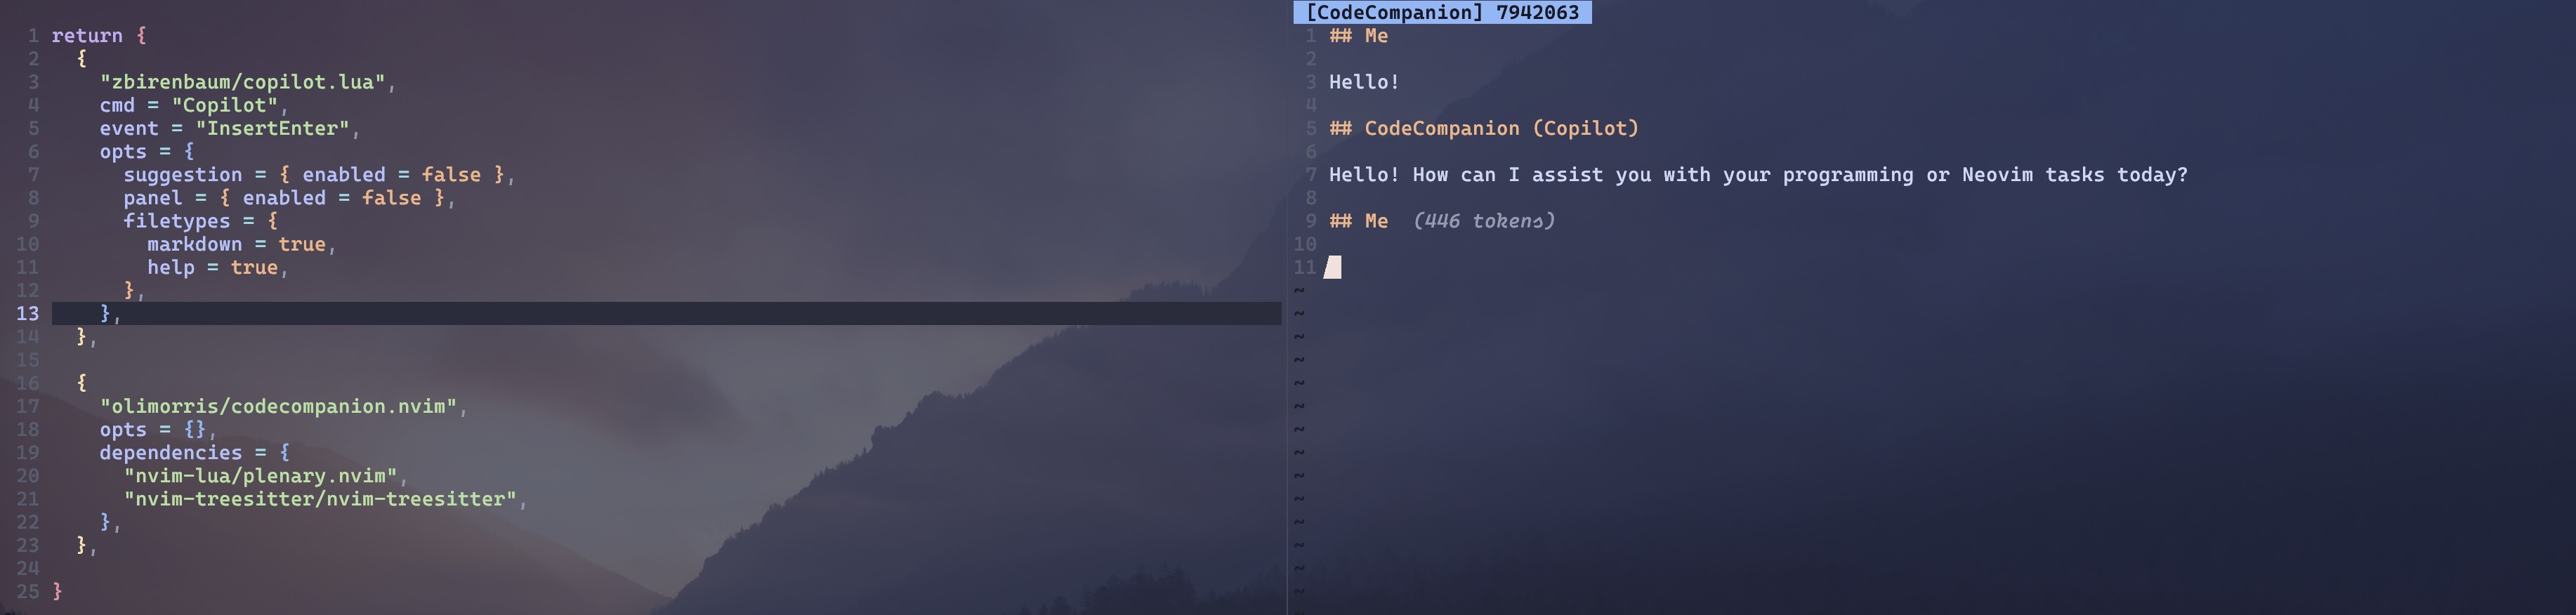
\includegraphics[width=\linewidth]{./Figures/CodeCompanion_Instal_Result.jpg}
          \end{figure}
      \end{itemize}
    \end{frame}

\section{插件配置}
  \begin{frame}{插件配置}
    \begin{itemize}
      \item 配置文件目录:\lstinline[language={}, style=path]{\~/.config/nvim/lua/plugins/ai.lua}

      \item 美化插件:
        \begin{itemize}
          \item \link{copilot-lualine}{https://github.com/AndreM222/copilot-lualine}:在lualine中显示Copilot的状态
          \item \link{mini.diff}{https://github.com/echasnovski/mini.diff}:更好地显示CodeCompanion对代码的修改 % ChkTeX 19
        \end{itemize}
    \end{itemize}
  \end{frame}

  \begin{frame}
    \begin{itemize}
      \item 感谢:
        \begin{itemize}
          \item \link{Catppuccin}{https://catppuccin.com/} 
\includegraphics[height=10pt]{./Figures/Catppuccin_logo.png}
          \item \link{Catppuccin for beamer}{https://github.com/atticus-sullivan/beamercolortheme}
        \end{itemize}
        \vspace{0.5cm}
      \item 本教程的全部材料可以在我的Github上找到
        \begin{itemize}
          \item Slides: \url{https://github.com/Jacky-Lzx/nvim.tutorial.slides}
          \item Config: \url{https://github.com/Jacky-Lzx/nvim.tutorial.config}
        \end{itemize}
    \end{itemize}
  \end{frame}

\end{document}
